\documentclass[10pt,xcolor={dvipsnames}]{beamer}
\usetheme[progressbar=frametitle, block=fill]{metropolis}
\usepackage{listings}
\usepackage{pgfpages}
\usepackage{pifont}
\usepackage{amsmath}
\usepackage{amsfonts}
\usepackage{amssymb}
\usepackage{tikz-uml}
\usepackage{csquotes}
\usepackage{caption}

\DeclareCaptionFormat{myformat}{#3}
\captionsetup{format=myformat}

\newcommand{\tmark}{$\thicksim$}
\newcommand{\cmark}{\ding{51}}
\newcommand{\xmark}{\ding{55}}

\setbeamertemplate{caption}{\raggedright\insertcaption\par}
\setbeamertemplate{section in toc}[sections]
\setbeamercovered{invisible}
%\setbeameroption{show notes on second screen=bottom}

\author{Dominik Moser}
\date{October 3\textsuperscript{rd}, 2017}
\title{Java 9}
\usepackage{fontspec}
\setmonofont[
Contextuals={Alternate}
]{Fira Code}

\lstset{%
	language=Java,
	basicstyle=\scriptsize\ttfamily,%
	numbers=left, numberstyle=\tiny, stepnumber=1, numbersep=10pt,%
	showstringspaces=false
	tabsize=4,
	captionpos=b,
	breaklines=true,
	breakatwhitespace=false,
	keywordstyle=\color{MidnightBlue}\ttfamily,
	stringstyle=\color{ForestGreen}\ttfamily,
	commentstyle=\color{RedOrange}\ttfamily,
	xleftmargin=0.5cm
}%

\lstdefinelanguage{module}{
	keywords={exports, uses, to, opens, requires, module},
}


%\titlegraphic{\vspace{.1\textheight}\includegraphics[height=.125\textheight]{figures/kotlinLogo2}}
\begin{document}
{
	\title{Java 9}
	\subtitle{for developers}
	\maketitle
}
\begin{frame}{Table of contents}
 \begin{columns}
 	\begin{column}{.45\textwidth}
 		\fontsize{10}{18}\selectfont
		\tableofcontents[sections=1-5]
	\end{column}
	\begin{column}{.45\textwidth}
		\fontsize{10}{18}\selectfont
		\tableofcontents[sections=6-10]
	\end{column}
\end{columns}
\end{frame}
\section{Modularisation}

\begin{frame}{Modularisation: Jigsaw}
	\begin{quote}
		\enquote{\dots \textbf{unnamed module} reads every other module. \dots able to access the exported types of all other readable modules, which by default will include all of the named, built-in platform modules.}
	\end{quote}
	\begin{quote}
		\enquote{\dots placing it, unmodified, on the module path rather than the class path. \dots \textbf{automatic module} is a named module that is defined implicitly, since it does not have a module declaration.}
	\end{quote}
	\begin{quote}
	\enquote{
		\dots ordinary named module, \dots is defined \textbf{explicit}ly, with a \textbf{module} declaration}
	\end{quote}
\end{frame}

\begin{frame}{Modularisation: Jigsaw}
\lstinputlisting[language=module,caption=module-info.java]{./code-sample/modular.universe/ui/src/main/java/module-info.java}
\end{frame}

\begin{frame}[fragile]{Docker Support: Minimizing Image Size}
\begin{onlyenv}<1>
	\fontsize{20}{0}\selectfont
	\hfill DEMO \hfill
\end{onlyenv}
\begin{onlyenv}<2>
\begin{lstlisting}[language=, caption=Minimizing the JDK]
docker run --rm --volume $(pwd):/out java9-full \
    /bin/bash -c "jlink \
        --module-path /jdk-9/jmods \
        --verbose \
        --add-modules java.base \
        --compress 2 \
        --no-header-files \
        --output /out/jdk-mini && \
        chown -R 1000 /out/jdk-mini/"
\end{lstlisting}
\begin{lstlisting}[language=, caption=Resulting minimized image size]
java9-mini   latest   88de1   154MB
java9-full   latest   87542   688MB
ubuntu       latest   8b72b   120MB
\end{lstlisting}
\end{onlyenv}
\end{frame}

\section{Java + REPL = JShell}

\begin{frame}[fragile]{Java + REPL = JShell}
\textbf{R}ead \textbf{E}valuate \textbf{P}rint \textbf{L}oop
\begin{lstlisting}[language=, caption=JShell Sample Output]
$ jshell
|  Welcome to JShell -- Version 9
|  For an introduction type: /help intro

jshell> System.out.println(1 + 2)
3
jshell> import java.io.File;
jshell> new File("./foo.txt").createNewFile()
$3 ==> true
\end{lstlisting}
\end{frame}

\section{Garbage Collector}

\begin{frame}{Garbage Collector: Parallel to G1}
	\begin{itemize}
		\item Low pause collector
		\item \enquote{Pause Time Goal} defaults to 200ms
		\begin{itemize}
			\item Higher pause goal (more throughput, higher latency)
			\item Lower pause goal (less throughput, lower latency)
		\end{itemize}
		\item Runs on application thread
		\item Should not effect you
		\item Except you are dealing with high performance applications
		\item Different GCs
		\begin{itemize}
			\item Serial (Memory Footprint)
			\item Parallel (Throughput)
			\item CMS (Latency)
			\item G1 (Throughput / Latency Balance)
		\end{itemize}
	\end{itemize}
\end{frame}

\section{Collections}

\begin{frame}[fragile]{Collections: \dots.of(\dots)}
\begin{onlyenv}<1>
	\fontsize{20}{0}\selectfont
	\hfill DEMO \hfill
\end{onlyenv}
\begin{onlyenv}<2>
	\lstinputlisting[language=java,firstline=9,lastline=23,caption=Maps in Java8]{./code-sample/simple/src/main/java/rtt/java9/code/sample/simple/collections/Java8Map.java}
\end{onlyenv}
\begin{onlyenv}<3>
	\lstinputlisting[language=java,firstline=10,lastline=26,caption=Collections in Java9]{./code-sample/simple/src/main/java/rtt/java9/code/sample/simple/collections/Java9Collections.java}
\end{onlyenv}
\end{frame}

\section{Publish-Subscribe}

\begin{frame}{Publish-Subscribe: Reactive Streams}
Existing Implementations of Reactive Streams
	\begin{itemize}
		\item Akka
		\item Reactor
		\item RxJava
		\item \dots
	\end{itemize}
\end{frame}

\begin{frame}{Publish-Subscribe: Reactive Streams}
	\begin{figure}[h]
		\centering
		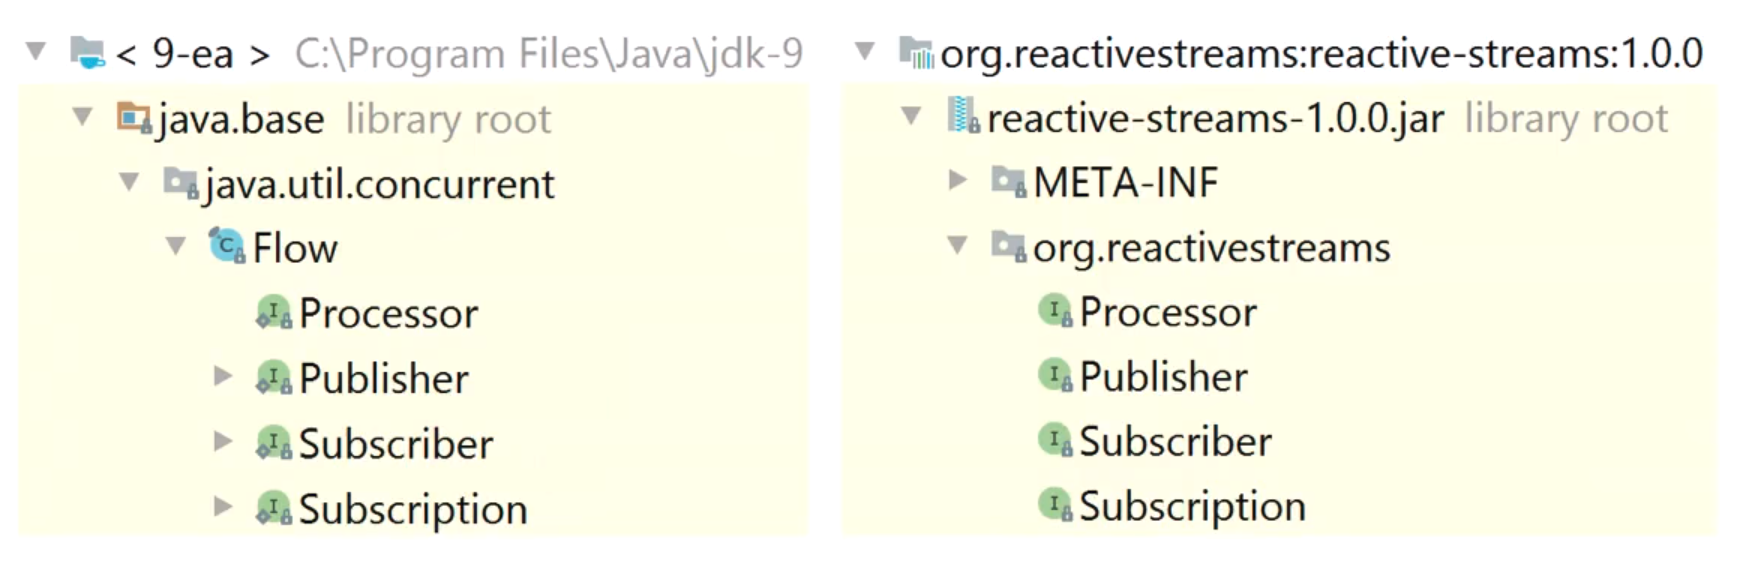
\includegraphics[width=\textwidth]{./figures/reactiveStreams.png}
		\caption{Reactive Steams, Java VS. org.reactivestreams}
	\end{figure}
	Thinks to note:
	\begin{itemize}
		\item Popular implementations will probably adapt quickly 
		\item \enquote{Java 8} Streams are not equal to Reactive Streams,\\
				so don't mess up those two things
	\end{itemize}
\end{frame}

\begin{frame}[fragile]{Publish-Subscribe: Reactive Streams}
\begin{onlyenv}<1>
	\fontsize{20}{0}\selectfont
	\hfill DEMO \hfill
\end{onlyenv}
\begin{onlyenv}<2>
	\lstinputlisting[language=java,firstline=10,lastline=31,caption=SampleSubscriber]{./code-sample/simple/src/main/java/rtt/java9/code/sample/simple/reactive/PublisherSubscribe.java}
\end{onlyenv}
\begin{onlyenv}<3>
\lstinputlisting[language=java,firstline=33,lastline=49,caption=Using the SampleSubscriber]{./code-sample/simple/src/main/java/rtt/java9/code/sample/simple/reactive/PublisherSubscribe.java}
\end{onlyenv}
\end{frame}

\section{Other Cool Stuff}

\begin{frame}{Other Cool Stuff}
	\begin{itemize}
		\item A New HTTP Client (HTTP/2)
		\item Try-With-Resources
		\item Diamond Operator Extension
		\item Process API
		\item Interface Private Method
		\item Improved Optional Support (ifPresentOrElse)
		\item Stream Improvements (takeWhile \& dropWhile \& iterate)
		\item \enquote{Modern} JavaDoc
	\end{itemize}
\end{frame}

\section{Release Model}

\begin{frame}{Release Model}
	Oracle JDK \& Open JDK
	\begin{figure}[h]
		\centering
		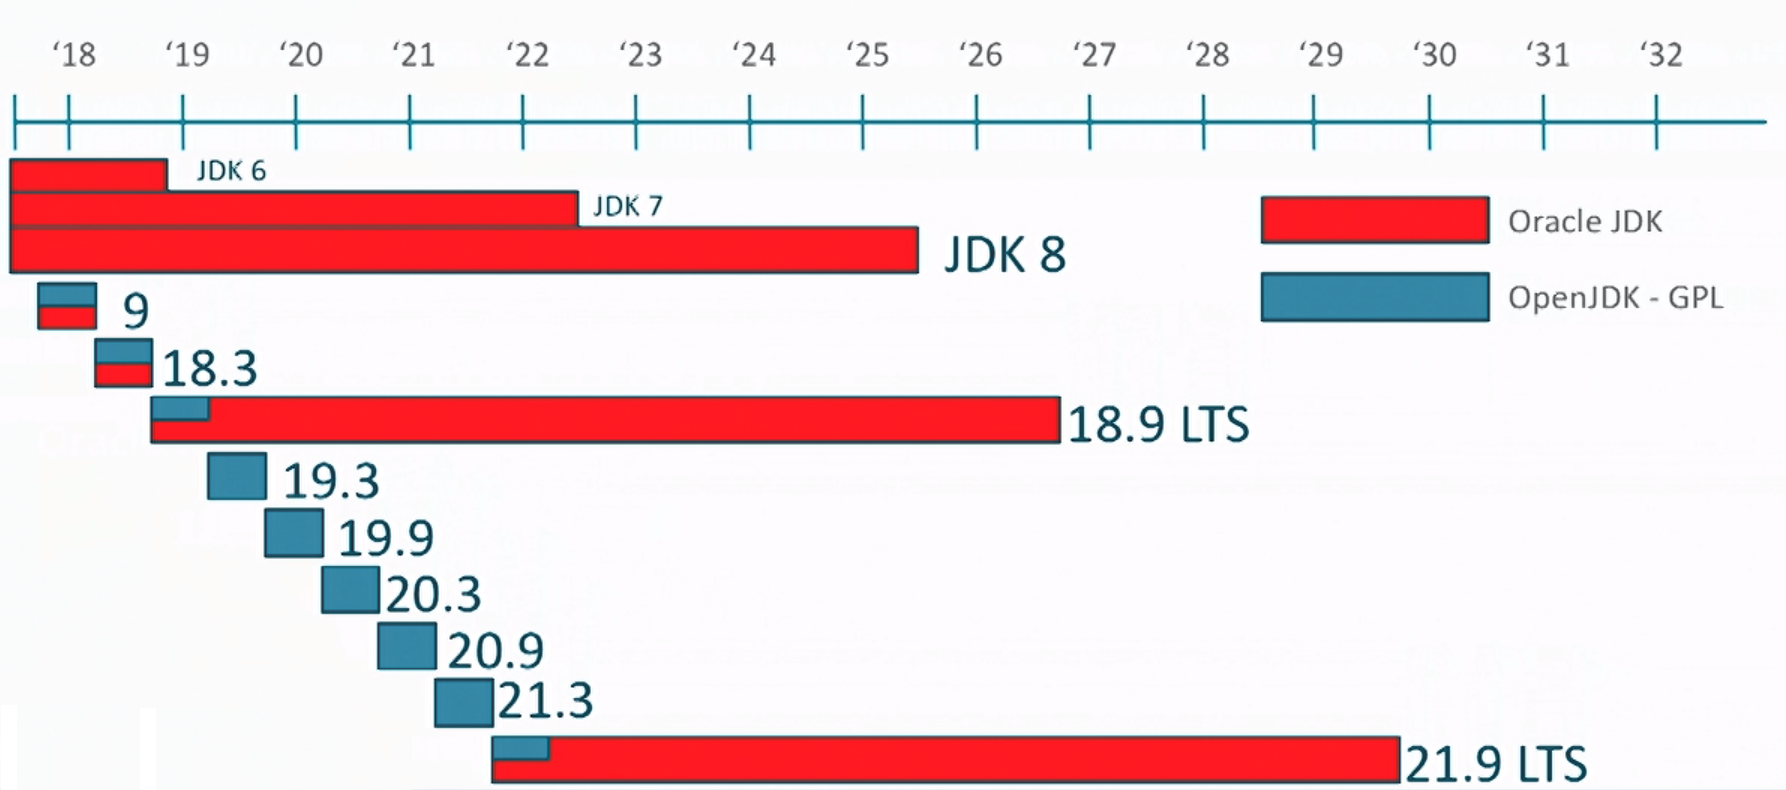
\includegraphics[width=\textwidth]{./figures/releaseModel.png}
		\caption{New JDK Release Model}
	\end{figure}
\end{frame}

\section{Things you get for free}

\begin{frame}{Free Stuff}
	\begin{itemize}
		\item Better Memory Usage (i.e. Strings)
		\item Better Security (JKS to PKCS12, SHA3)
		\item Better Performance
		\begin{itemize}
			\item Locking
			\item Graphics
		\end{itemize}
		\item Better Use of Hardware
		\item Better Documentation
		\item Better Deprecations
		\item Prettier Graphics (HiDPI on Windows \& Linux)
		\item Faster Compilation
		\item Multi Release JAR Files
	\end{itemize}
\end{frame}

\section{Uncovered}

\begin{frame}{Uncovered}
	\begin{itemize}
		\item Java8 EE
		\item Better ARM Support
		\item Stack-Walking API
		\item Some of the 91 JEPs (JDK Enhancement Proposals)
		\begin{itemize}
			\item Full list: \url{http://openjdk.java.net/projects/jdk9/}
		\end{itemize}
	\end{itemize}
\end{frame}


\section{Production}

\begin{frame}{Production}
\centering
\fontsize{20}{0}\selectfont
\onslide<1->{Is it ready for Production?\\}
\vspace{0.5cm}
\fontsize{20}{0}\selectfont
\onslide<2->{\alert{\textbf{With Caution!}}}
\end{frame}

\begin{frame}{Production}
	\begin{itemize}
		\item[\textcolor{ForestGreen}{\cmark}] Jigsaw In New Projects
		\item[\textcolor{Orange}{\xmark}] Migrating Old Projects
		\item[\textcolor{ForestGreen}{\cmark}] Framework Support (Spring, SLF4J, \dots)
		\item[\textcolor{Orange}{\xmark}] Framework Support (Project Lombok, upgrades!, \dots)
		\item[\textcolor{ForestGreen}{\cmark}] The Cool New Stuff (Collections, Publish-Subscribe, \dots)
		\item[\textcolor{Orange}{\xmark}] The Cool New Stuff (HTTP/2, incubating!, \dots)
		\item[\textcolor{ForestGreen}{\cmark}] G1 Garbage Collector
		\item[\textcolor{Orange}{\xmark}] G1 Garbage Collector (High Performance)
		\item[\textcolor{ForestGreen}{\cmark}] Tool Support (works in IntelliJ)
		\item[\textcolor{Orange}{\xmark}] Tool Support (but still evolving, EA)
	\end{itemize}
\end{frame}

\begin{frame}[standout]
\fontsize{20}{0}\selectfont
Thank You!\\
\vspace{0.5cm}
\fontsize{10}{0}\selectfont
You can find all samples at\\
\vspace{0.5cm}
\url{https://github.com/hemeroc/rtt-java9}\\
\vspace{0.5cm}
\fontsize{20}{0}\selectfont
Questions?
\end{frame}

\end{document}